\section{Letter Font Application}
\label{sec:font}
This section presents the letter and font GUI application, the input comes from a user, and the user can choose a set of settings, the main settings are the font, font style and font size. This application writes a set of milling points to an output .txt file. The letter font model is implemented under vision (image processing), so all theory from image processing could be applied there.\\
The purpose of this application is to return letters milling points, and these milling points would be used to performing milling (carving) by the robot arm Fanuc 200ib (figure \ref{fig:writingbox}).

\begin{figure}[H]
  \centering
  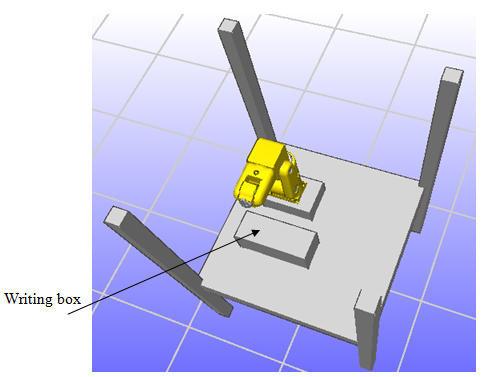
\includegraphics[scale= 1]{source/writingbox.png}
  \caption{Writing box position}
  \label{fig:writingbox}
\end{figure}

Letter font model is an important step for performing actual (real) letter carving in foam, another step would be inverse kinematics, which the path planner uses for planning movements between frames. The applications main window is shown in figure  \ref{fig:letterapp}, there are also provided a description of the application elements.

\begin{figure}[H]
  \centering
  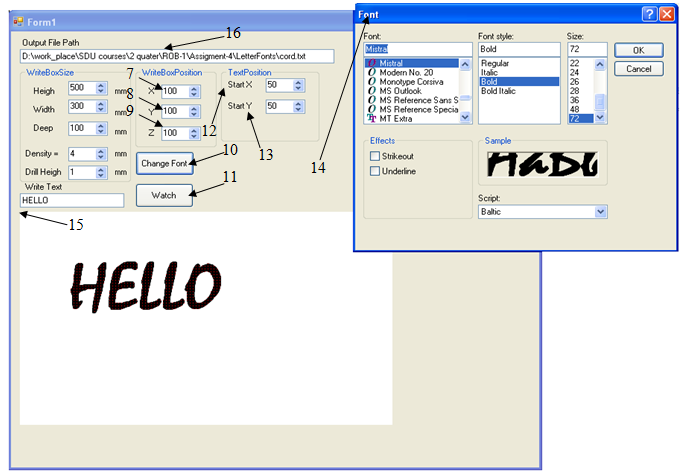
\includegraphics[scale= 0.8]{source/letterapp.png}
  \caption{Letter font application}
  \label{fig:letterapp}
\end{figure}

\begin{enumerate}
\item Sets writing box height
\item Sets writing box width
\item Sets writing box deep
\item Set the density of drilling points (red points)
\item Sets the drill height, in other words, how deep we want to drill
\item The place of letter or text
\item Set the writing box position according X coordinate (in Cartesian domain)
\item Set the writing box position according Y coordinate (in Cartesian domain)
\item Set the writing box position according Z coordinate (in Cartesian domain) 
\item Call the font window
\item Display the text on writing box
\item Set the text position according X (in Cartesian domain) on writing box
\item Set the text position according Y (in Cartesian domain) on writing box
\item The font window, where we can the size, font, font style of text
\item The start position of writing box
\item The path of txt file, where all the milling points are stored
\end{enumerate}
The text fields have been changed to make the understanding of the application easier, for an updated picture see figure \ref{fig:LetterFontsFinal} in appendix.

The default output path for the generated .txt file is the same directory as the application directory but can be changed to a user defined. The output file stores all the milling points, this information can also be seen in the C\# application (figure \ref{fig:letterconsole}). Second it is necessary to set the writing box position, because according to this position, is where the milling points start, and the other settings are optional. The density option is also written to the output file because it is used by the RobWorkStudio plugin to find the gaps in the letters and of course also to define how exact the milling tool will follow the letters outlines.

\begin{figure}[H]
  \centering
  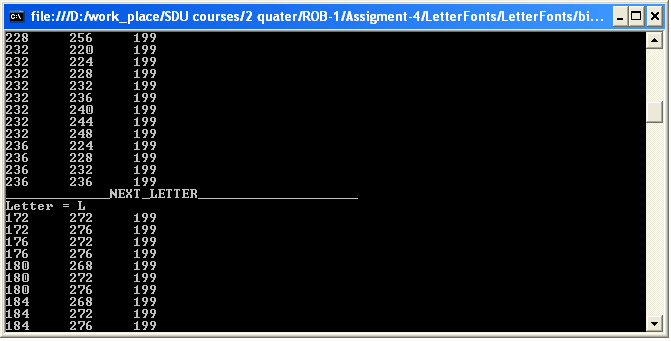
\includegraphics[scale= 0.6]{source/letterconsole.png}
  \caption{Letter font application console}
  \label{fig:letterconsole}
\end{figure}

As it can be seen in figure \ref{fig:letterconsole} each letter will be milled until it is finished before it begins on a new one. If this weren't the case the milling tool would never know when a new letter had begun and wouldn't rise the tool to start at the new starting point.

\subsection{Letter labeling application}
The image is dealt with in byte mode and the image is represented like a figure \ref{fig:imagebyte}. As we can see the image is composed of R-red, G-green, B-blue bytes and padding bytes. The only thing that is interesting are RGB bytes, the padding bytes describes how the image is stored in memory, and they do not have any influence of displaying the image. The programming becomes complex, because in order to jump to the next image row we need the count offset (which is equal to (stride - image width)), and in order to access the next pixel we need to jump three bytes.

\begin{figure}[H]
  \centering
  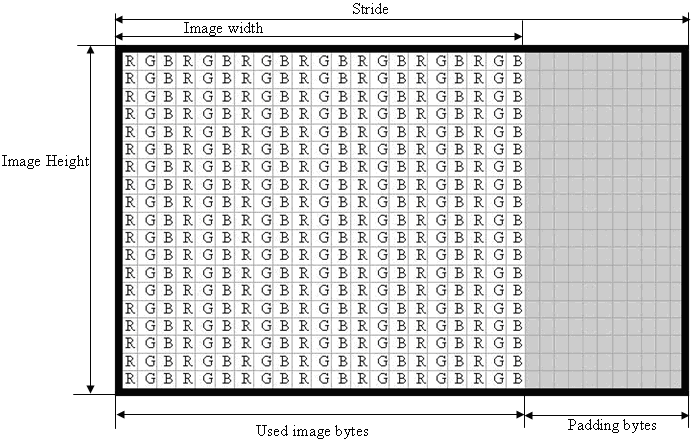
\includegraphics[scale= 0.6]{source/imagebyte.png}
  \caption{Image in byte mode}
  \label{fig:imagebyte}
\end{figure}

There are two images, one image is the original, and the other image is a clone of the original one. In the clone image each pixel bytes are accessed as an array, where the values are changed, it's done
so, because it is faster, and easier to access to write values, rather than to create a huge array.

A 8-connectivity matrix were used see figure \ref{fig:pixelmatrix}, there are a lot of options but this one were chosen, it is not too big and it is easy to manage this type of matrix (not like triangles or cross shape).  

\begin{figure}[H]
  \centering
  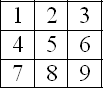
\includegraphics[scale= 0.6]{source/pixelmatrix.png}
  \caption{9 pixel connectivity matrix}
  \label{fig:pixelmatrix}
\end{figure}

The connectivity matrix is used to take values from the original image and write the result to a clone image. Another reason of choosing 3x3 connectivity matrix is that we loose only the images corner pixels. It was a possibility to choose 2x2 matrix, but the time of image processing would increase significantly, and the corner pixels would also be lost in the process.

\begin{figure}[H]
  \centering
  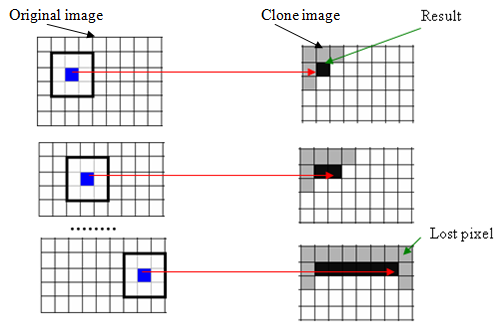
\includegraphics[scale= 0.6]{source/matriximages.png}
  \caption{9 pixels connectivity matrix over image}
  \label{fig:matriximages}
\end{figure}

The letters (objects) labeling algorithm is shown in figure \ref{fig:matriximages}. At the beginning the image is converted to binary, it made it easier to deal with the information, non-white pixels were set to black. 

\begin{figure}[H]
  \centering
  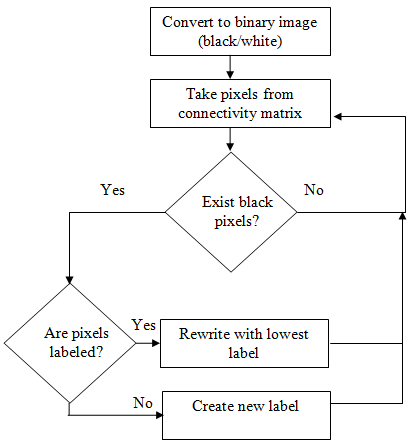
\includegraphics[scale= 0.6]{source/labeling.png}
  \caption{Letters labeling algorithm}
  \label{fig:labeling}
\end{figure}

When a binary image is used there are only two values: black which represent the letter (or object), and white which are assumed to be the background. In the next step, pixels from the connectivity matrix are looked at and a check if black pixels (which belongs to letter or object) exists are done. If there are no black pixels, a move of the connectivity matrix by one pixel in a particular direction and a repeat of the black pixel checking are done. But if there are black pixels, a check are performed in order to figure out if a new label (detected new object) needs to be created, or some of these pixels belongs to a previously detected letter (or object), and it is enough to rewrite the previous labels. The example of labeling text letters is shown in figure \ref{fig:labelingexample}. We have a binary image this image is called "clone image"� it is a copy of the original. By performing the letter labeling algorithm (figure \ref{fig:labeling}) a detection of how many different letters (objects) there are can be done. The important thing is that the letter labeling algorithm are repeated twice, at first time it's arbitrarily chosen which corner of the image where the algorithm starts, for instance it's convenient to start in the top/left corner, when the algorithm repeats an opposite corner is chosen to start from, it could be the bottom/right one.

\begin{figure}[H]
  \centering
  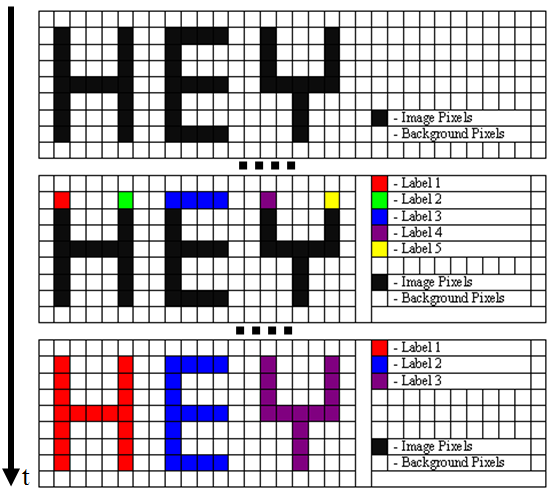
\includegraphics[scale= 0.6]{source/labelingexample.png}
  \caption{Letters labeling example}
  \label{fig:labelingexample}
\end{figure}

If the algorithm wouldn't start from the opposite corner, the algorithm would detect more letters (objects) then there exists, in such letters as U, Y, H, V, W... , because the connectivity matrix is too small, but if a connectivity matrix was chosen to be quite large, there are risks: i.e. detect two letters as one letter, loose more pixels (near image corners).

\subsection{Letter Font Application Extension}
At the moment the letter font application deals with text as an image, in other words, the letters are consider as an image (which can be saved, painted or color changed). It is possible to load an image directly (this feature is not implemented on final application, because the task was to deal with letters), so by using this application source code and knowing the basics of object oriented programming, it's easy to load any picture here as shown in figure \ref{fig:letterappextension}.   

\begin{figure}[H]
  \centering
  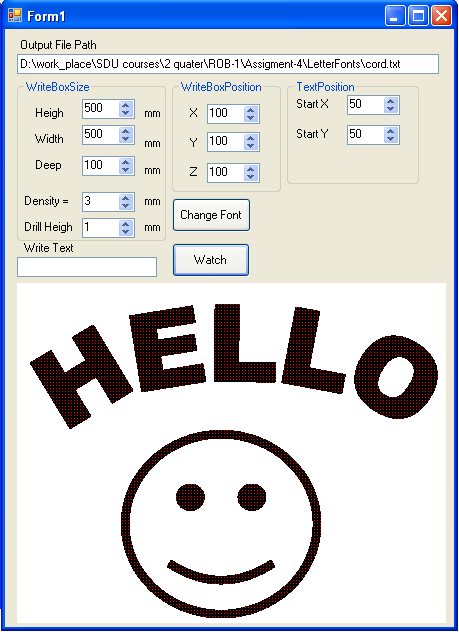
\includegraphics[scale= 0.6]{source/letterappextension.png}
  \caption{Letter font application}
  \label{fig:letterappextension}
\end{figure}

What is interesting is that more image processing knowledge could be applied here, such as edge detection, Hough transformation etc., and this mean that this letter font application is universal, we can easy make extensions.  
